\documentclass[12pt,a4paper]{article}
\usepackage[utf8]{inputenc}
\usepackage[french]{babel}
\usepackage[T1]{fontenc}
\usepackage{amsmath}
\usepackage{amsfonts}
\usepackage{amssymb}
\usepackage{graphicx}
\usepackage{url}
\usepackage[usenames,dvipsnames]{xcolor}
\usepackage[colorlinks=false,urlbordercolor=white,linkbordercolor=white]{hyperref}
\usepackage[left=2cm,right=2cm,top=2cm,bottom=3cm]{geometry}
\usepackage{fancyhdr}
\usepackage{lmodern}
\usepackage{hyperref}
\usepackage{listings}
\pagestyle{fancy}
\usepackage{titlesec}
\usepackage[abs]{overpic}
\usepackage{tabularx}
\usepackage{times}
\usepackage{tikz}
% gestion de la police sans-serif (helvetica, équivalent arial) :
% décommenter les deux lignes suivantes
%\usepackage{helvet}
%\renewcommand{\familydefault}{\sfdefault}

% Definition de l'affichage du code
\lstset{breaklines=true,basicstyle=\footnotesize\ttfamily,frame=single, numbers=left
%,backgroundcolor=\color{lightgray}
}

% Definition des couleurs
\definecolor{titreColor}{RGB}{0,58,128}  % Marine
\definecolor{stitreColor}{RGB}{0,158,224}  % Ocean
\definecolor{auteurColor}{RGB}{0,58,128}     % Marine
\definecolor{texteColor}{RGB}{164,196,0}     % Prairie

% Definition du sommaire
\usepackage[tight]{shorttoc}
\newcommand{\sommaire}{\shorttoc{Sommaire}{2}}

% Definition des chapitres
\titleformat{\section}
{\color{titreColor}\normalfont\Large\bfseries\sffamily}
{\color{titreColor}\thesection}{1em}{}

\titleformat{\subsection}
{\color{stitreColor}\bfseries\sffamily}
{\color{stitreColor}\thesubsection}{1em}{}

%Données de titre et d'auteur pour la page de garde
\newcommand{\titre}{Cas d'utilisation pour le projet sturwild}
\newcommand{\auteur}{Maxime Boisse}
\newcommand{\dateModif}{\today}

\begin{document}
%Supprime les veuves et orphelines
\widowpenalty=10000
\clubpenalty=10000
\raggedbottom 

%entete
\fancyhead{}
\renewcommand{\headrulewidth}{0pt}

%pied de page
\fancyfoot{}
\fancyfoot[C]{\sffamily\thepage}
\fancyfoot[L]{\textcolor{titreColor}{\sffamily\textbf{IRSTEA} - Centre de Bordeaux\\}
\fancyfoot[R]{\textcolor{auteurColor}{\sffamily\auteur{}}\\{\sffamily\dateModif{}}}
\textcolor{stitreColor}{\sffamily 50, avenue de Verdun, Gazinet\\
33612 CESTAS Cedex }}
\fancyfoot[R]{\sffamily\author{}}

% Insertion du logo, du titre et du sous-titre
\emph{\begin{minipage}{0.2\linewidth}
\includegraphics[width=3.06cm,height=9.57cm,keepaspectratio]{logo_irstea}%
\end{minipage}
\hspace{0.1cm}
\begin{minipage}{0.8\linewidth}
\LARGE\flushleft \color{titreColor}{\bfseries\sffamily\titre{}}\\
\end{minipage}}

% Insertion du sommaire
% \sommaire
%\tableofcontents

% Debut effectif du texte
\sffamily
\section{Présentation}
Le projet \textit{sturwild} s'inscrit dans le cadre d'un suivi des captures accidentelles d'esturgeons européens (\textit{Acipenser sturio}), principalement au niveau de l'estuaire de la Gironde. Cette action s'inscrit dans le plan national d'action (connu sous le nom de plan de restauration ou PNA) qui vise à conserver la population d'esturgeons européens à un niveau favorable. Ce PNA fait partie d'une action d'ampleur européenne de protection et de conservation des esturgeons européens.

Le pêcheur, qu'il soit amateur ou professionnel, doit de déclarer la prise d'un esturgeon. Les informations récoltées  lors de la déclaration peuvent être recueillies par différents organismes tels que le CNPMEM (\textit{Comité National des Pêches Maritimes et des  Marins}), l'IMA (\textit{l'Institut des Milieux Aquatiques}) ou Irstea. Une fois les déclarations saisies, elles sont transmises à Irstea. Après une phase de contrôle et de vérification effectuée par le responsable du projet, l'ensemble des informations obtenues sont traitées puis partagées avec tous les partenaires du PNA: l'IMA, le CNPMEM, Migado et la DREAL.
\clearpage

\section{Les cas d'utilisation}
\begin{figure}[h]
\centering
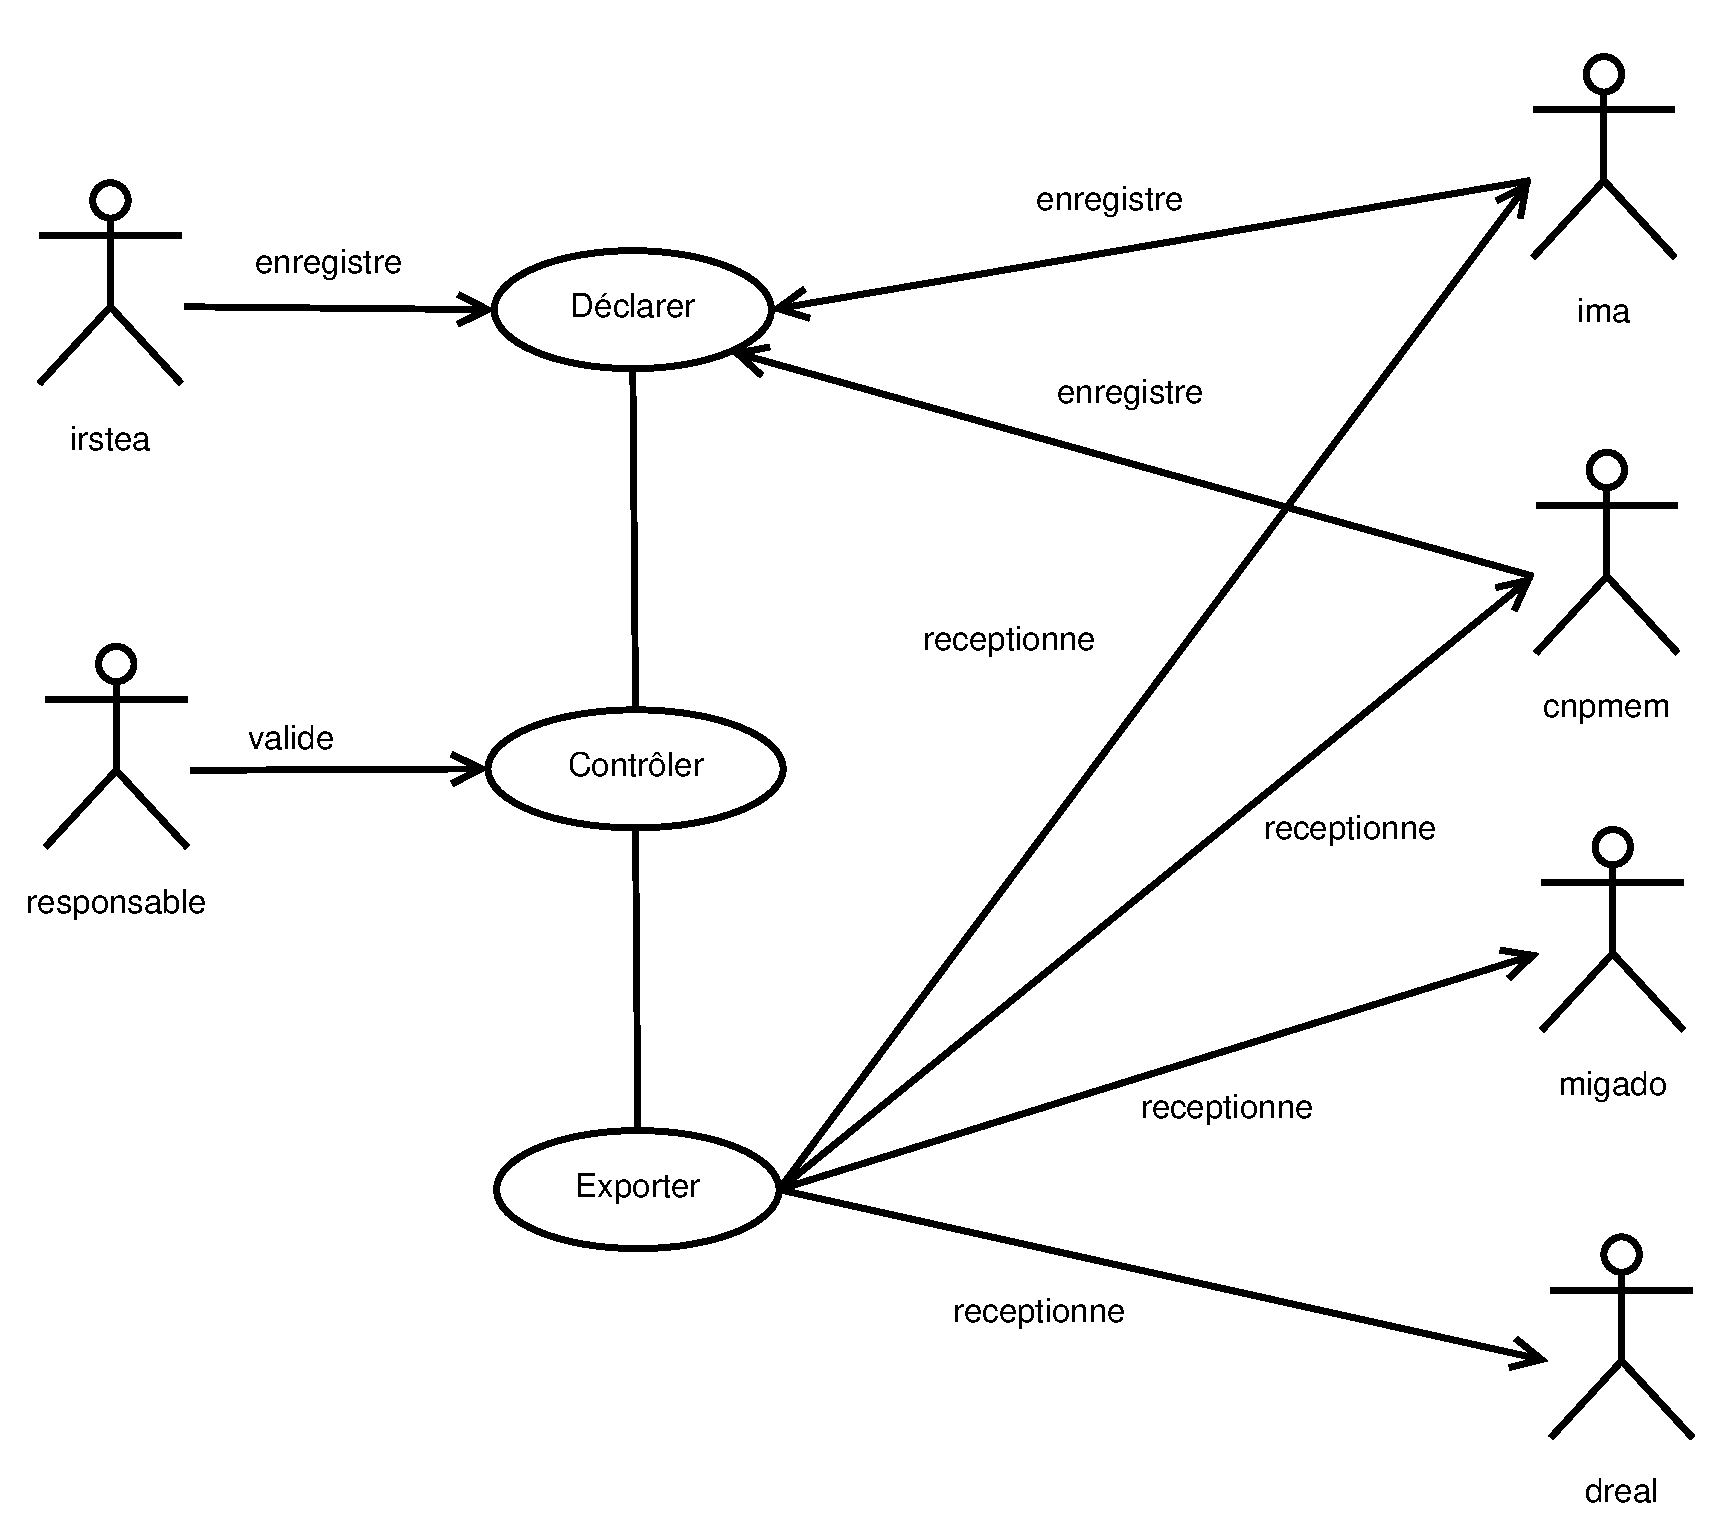
\includegraphics[width=\textwidth]{casUtilisation2.eps}
\caption{Diagramme des cas d'utilisation}
\end{figure}
\clearpage

\subsection{Déclarer}
\begin{figure}[h]
\centering
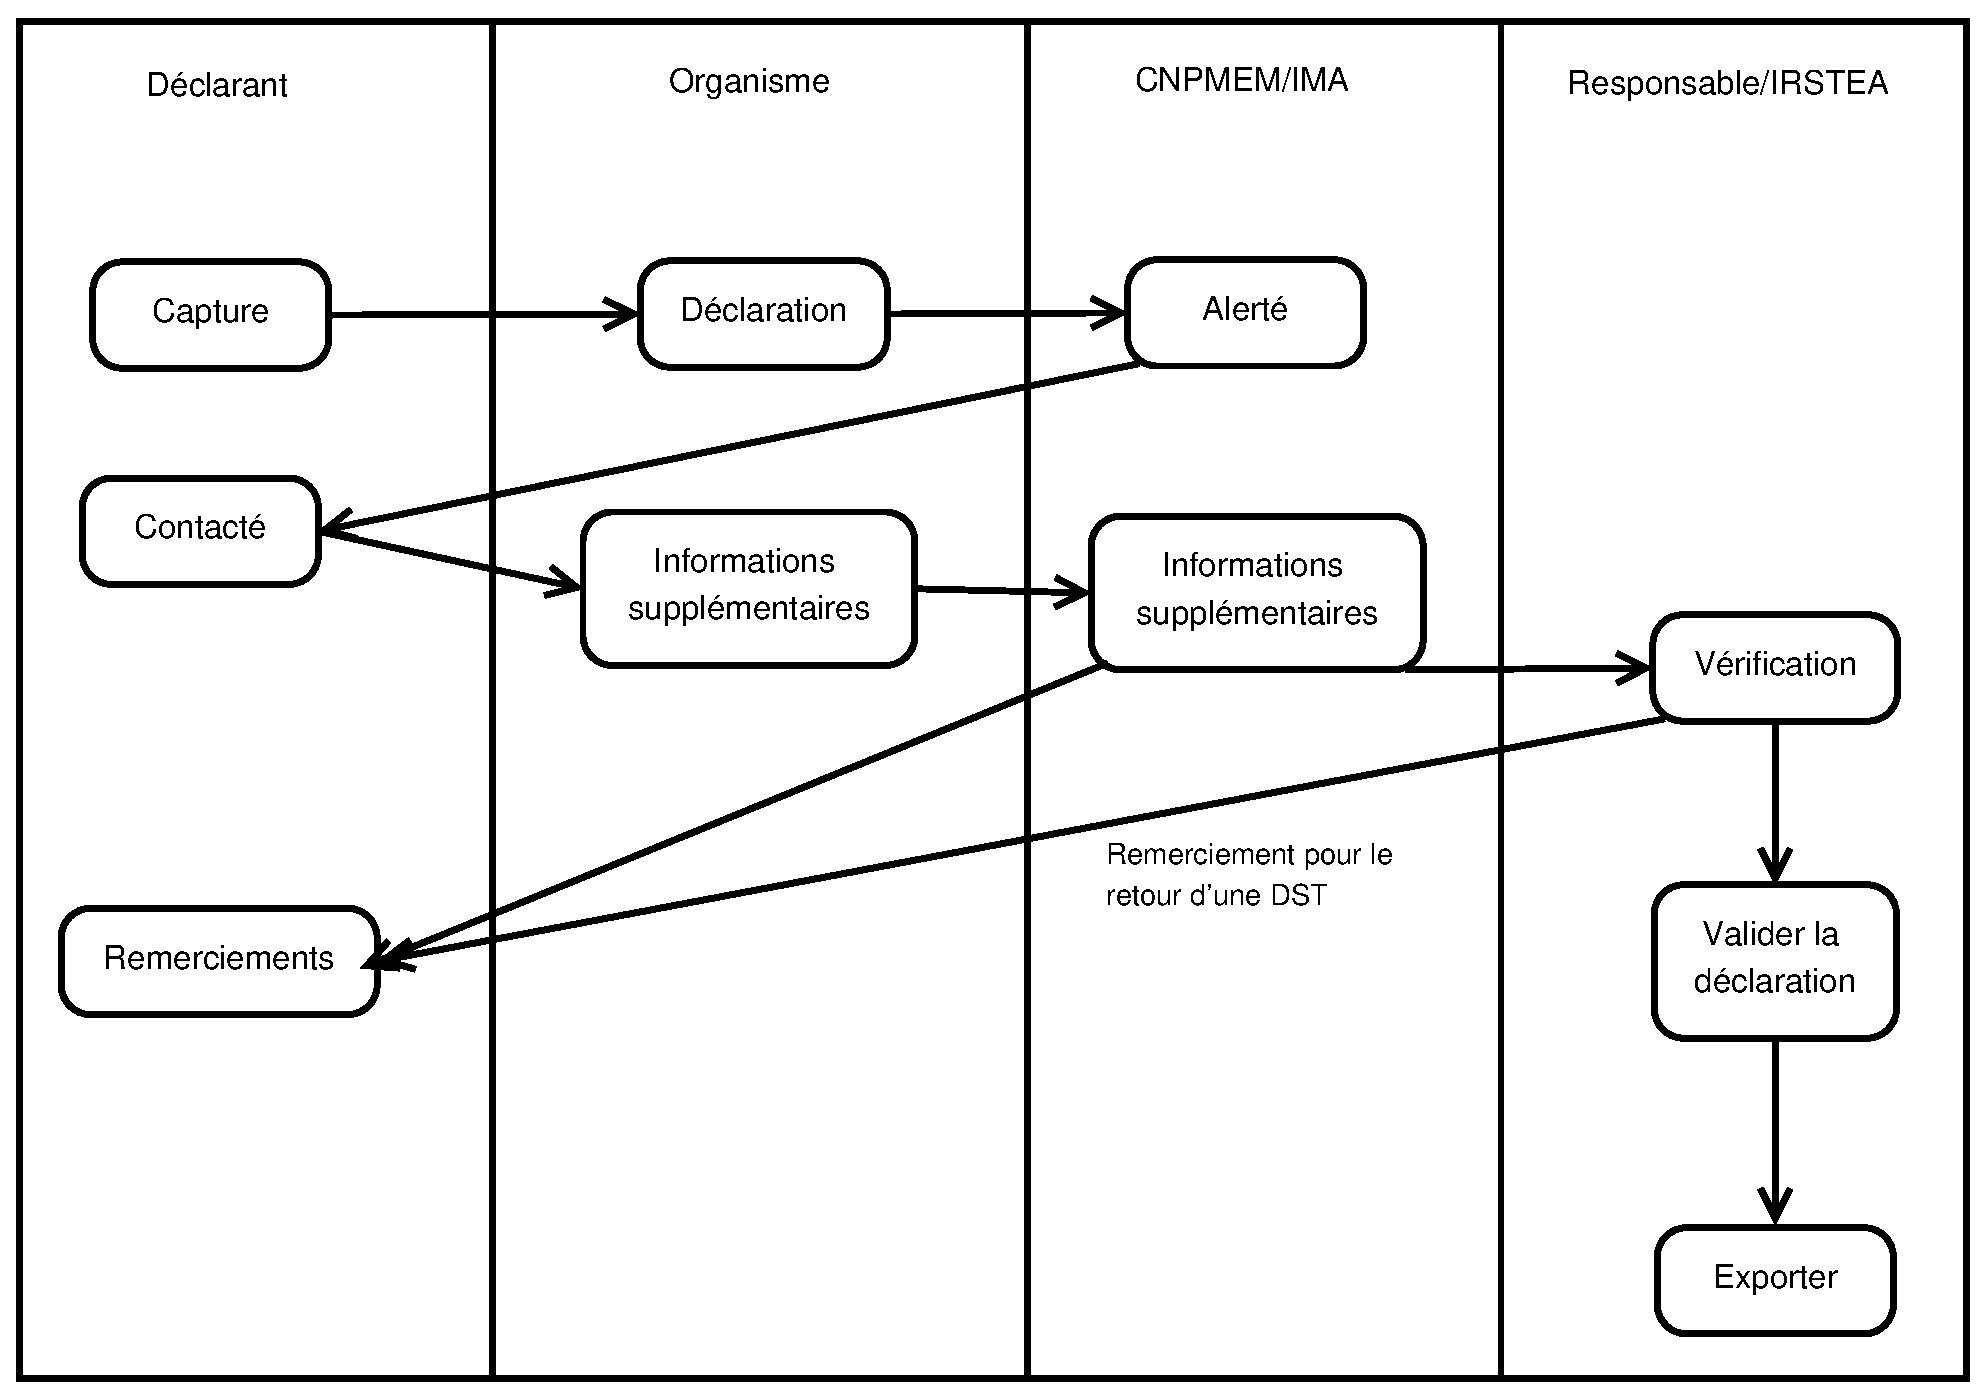
\includegraphics[width=\textwidth]{schemaDeclaration.eps}
\caption{Schéma de la déclaration}
\end{figure}
Un pêcheur peut signaler ses prises par l'intermédiaire de L'IMA, du CNPMEM Irstea. Une fois en relation avec un des organismes cités plus haut, le déclarant devra fournir les informations liées au mode de capture, à l'individu capturé et son état, au lieu de pêche. Il aura aussi la possibilité de joindre des photos à sa déclaration.

Afin que le pêcheur garde l'anonymat, le Comité des Pêches fournit un code qui remplace son identité vis-à-vis des autres organismes. En effet, le CNPMEM est le seul à détenir les noms des pêcheurs.  
De plus, il devra être averti pour toutes déclarations transmises par le pêcheur lui-même ou par un ou plusieurs intermédiaires.

Le site internet \url{www.sturio.eu} permet une déclaration spontanée des prises. Les coordonnées personnelles sont utilisées pour une reprise de contact. Les pêcheurs restent également anonymes sur le site.
\clearpage
\subsection{Contrôler}
\begin{figure}[h]
\centering
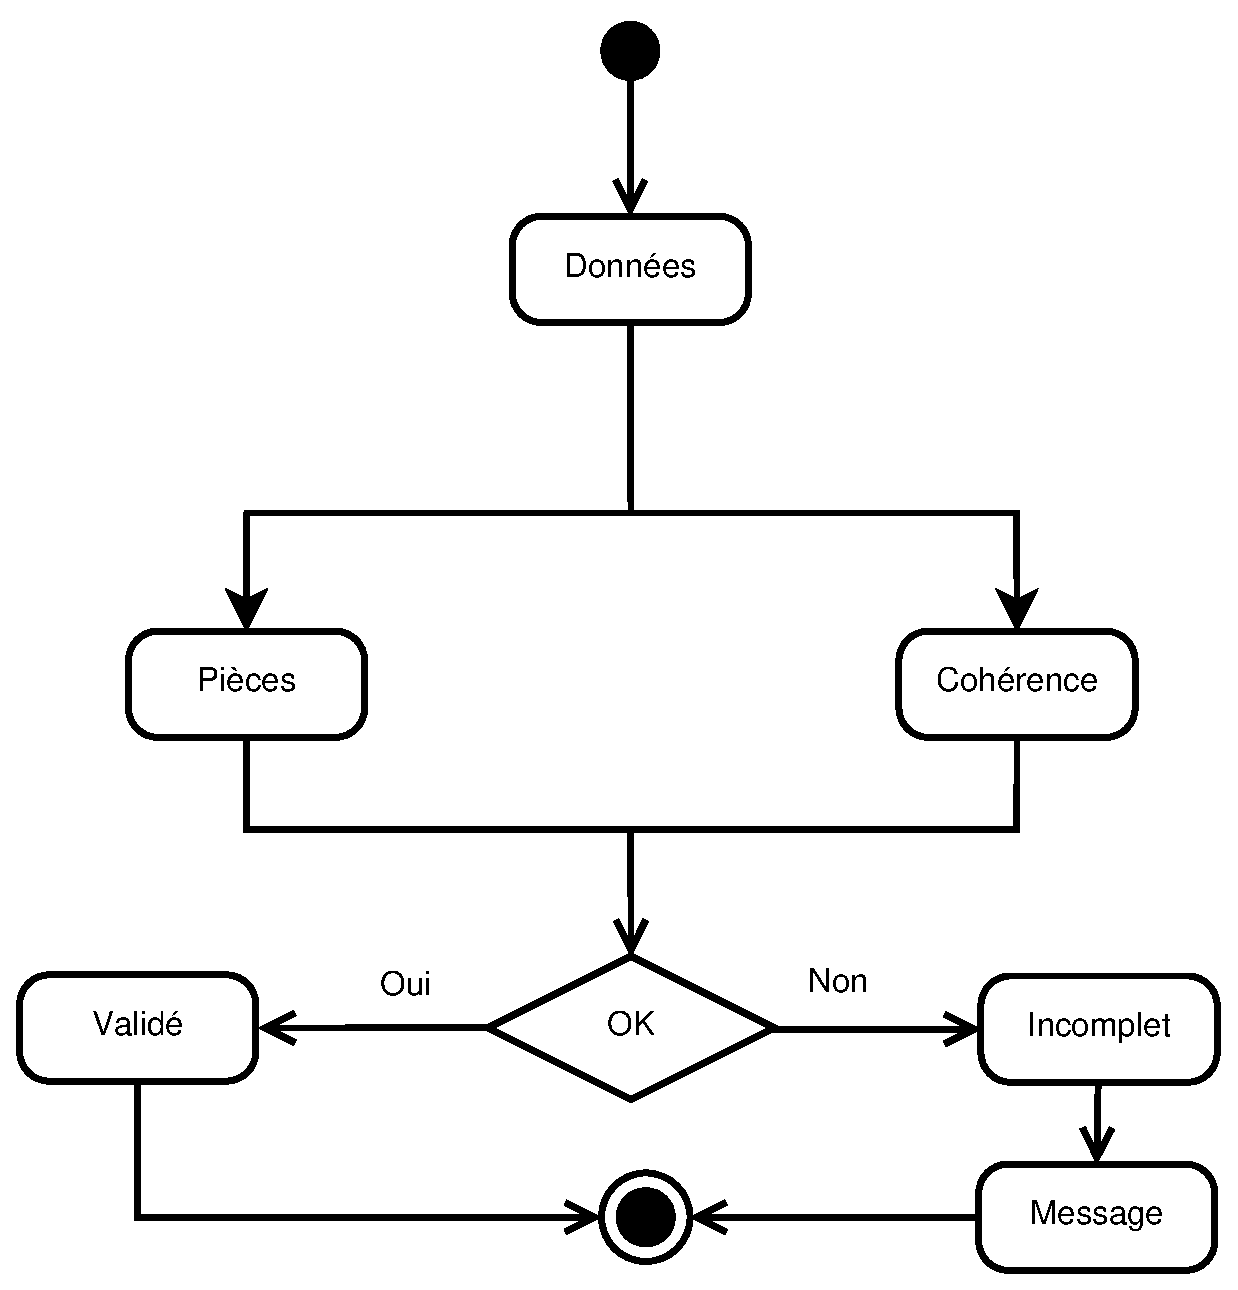
\includegraphics[width=\textwidth]{schemaControle.eps}
\caption{Schéma du contrôle}
\end{figure}
Le dossier possède un statut en fonction de son avancement, qui évolue au fur et à mesure de la progression des tests. Avant tout intervention du responsable, le dossier est "en saisie". Il doit encore être complété pour pouvoir être validé. Une fois arrivé en phase de tests, il a le statut "dossier saisi". Le responsable de la base intervient pour la suite de la procédure.

Le responsable contrôle la pertinence des pièces (photos, déclaration scannée) qui peuvent être liées à la déclaration. Il pourra ensuite vérifier la justesse et la cohérence des informations renseignées. 

Au terme de cette opération, le statut du dossier peut changer. Si le contrôle s'est bien passé, la déclaration sera validée. Sinon, elle est jugée incomplète et un message est envoyé à l'organisme qui s'est chargé de prendre la déclaration. 

\subsection{Exporter}

Environ tous les deux ou trois mois, ou sur demande, Irstea envoie la liste des captures enregistrées et validées à l'ensemble des partenaires du PNA. La version fournie par Irstea constitue la version officielle du PNA. 
Une date de dernière modification pourra être affichée sur les enregistrements des déclarations. 

\end{document}
